\documentclass{article}


\usepackage{PRIMEarxiv}

\usepackage[utf8]{inputenc} % allow utf-8 input
\usepackage[T1]{fontenc}    % use 8-bit T1 fonts
\usepackage{hyperref}       % hyperlinks
\usepackage{url}            % simple URL typesetting
\usepackage{booktabs}       % professional-quality tables
\usepackage{amsfonts}       % blackboard math symbols
\usepackage{nicefrac}       % compact symbols for 1/2, etc.
\usepackage{microtype}      % microtypography
\usepackage{lipsum}
\usepackage{fancyhdr}       % header
\usepackage{graphicx}       % graphics
\graphicspath{{Bilder/}}     % organize your images and other figures under media/ folder

% Einbinden von biblatex
\usepackage[backend=biber,style=numeric]{biblatex}
\addbibresource{Machine_Learning_Project.bib} % Lade die Bibliographie-Datei

%selber eingebunden
\usepackage[table]{xcolor}
\usepackage{colortbl}
\usepackage{float}
\usepackage{footmisc}
\usepackage{amsmath}
%Header
\pagestyle{fancy}
\thispagestyle{empty}
\rhead{ \textit{ }} 

% Update your Headers here
\fancyhead[LO]{Air Pollution Forecasting}
% \fancyhead[RE]{Firstauthor and Secondauthor} % Firstauthor et al. if more than 2 - must use \documentclass[twoside]{article}


%% Title
\title{Air Pollution Forecasting}

\author{
  Simon Spitzer \\
  business informatics student \\
  DHBW Stuttgart \\
  \texttt{simon.spitzer@live.de} \\
  \textbf{Projektdokumente Link: \href{https://github.com/Tzimon/Machine_Learning_Project_Semester_6}{Github Repository}}
  %% examples of more authors 
}


\begin{document}
\maketitle


\begin{abstract}
  Diese Studie entwickelt ein Framework zur Vorhersage von Luftverschmutzung mittels maschinellen Lernens.
  Basierend auf historischen Daten und meteorologischen Faktoren wird ein Modell trainiert und evaluiert.
  Das anschließend optimierte Modell zeigt eine hohe Vorhersagegenauigkeit und erfasst zeitliche Abhängigkeiten effektiv.
  Dieses Modell könnte so politische Entscheidungsträger und Umweltbehörden bei der Planung von Maßnahmen zur Luftqualitätskontrolle unterstützen.
\end{abstract}


% keywords can be removed
\keywords{Air Pollution Forecasting \and LSTM \and Regression \and MLFLow}



\section{Charakterisierung \& Aufbereitung Datensatz}
\subsection{Studienziel und Datensatz}
Diese Studie beschäftigt sich mit der Vorhersage von Luftverschmutzung einer US-Botschaft in Peking, China durch Einsatz maschinellen Lernens.\footcite[vgl.][1]{AirPollutionForecasting}
Der Datensatz streckt sich über fünf Jahre und enthält ca. 43.800 Datenpunkte, wobei jeder Datenpunkt einer stündlichen Aufnahme entspricht. 
Der vorherzusagende Wert ist die Luftverschmutzung, die als PM2.5-Konzentration angegeben wird und als Feinstaub bekannt ist.
Feinstaub bezeichnet Staubpartikel mit einer Korngröße von weniger als zehn Mikrometern.\footcite[vgl.][1]{bundesumweltministeriumsFeinstaub}
Der darin enthaltene PM2.5-Feinstaub trägt wesentlich zur Entstehung vieler Krankheiten bei.
Zu den negativen Folgen von PM2.5-Feinstaub gehören unter anderem Atemwegserkrankungen und Herz-Kreislauf-Erkrankungen.\footcite[vgl.][1]{FeinstaubPM2}
Das konkrete Ziel dieser Studie ist es, das Modell mit Daten der ersten vier Jahre zu trainieren, um die Luftverschmutzung im fünften Jahr möglichst genau vorherzusagen.
Im Detail wird in diesem fünften Jahr \textbf{immer der nachfolgende Tag vorhergesagt} mit dem Input von X Tagen in der vergangenheit, welche abhängig von der Batch Size sind.
Der benutzte Datensatz enthält dabei 9 verschiedene Eingabespalten ("Features"), die wie folgt aufgebaut sind:
\begin{table}[h!]
  \centering
  \begin{tabular}{|l|l|}
  \hline
  \textbf{Feature} & \textbf{Erklärung} \\ \hline
  Datum            & Datum in yyyy-mm-dd, hh:mm:ss \\ \hline
  Verschmutzung    & Luftverschmutzung in µg/m³ \\ \hline
  Taupunkt         & Taupunkt in °C \\ \hline
  Temperatur       & Temperatur in °C \\ \hline
  Druck            & Luftdruck in hPa \\ \hline
  Windrichtung     & Windrichtung, z.B. SE \\ \hline
  Windgeschwindigkeit & Windgeschwindigkeit in m/s \\ \hline
  Schnee           & Schneefall in mm \\ \hline
  Regen            & Regenfall in mm \\ \hline
  \end{tabular}
  \caption{Datenübersicht}
  \label{tab:datenuebersicht}
  \end{table} 

  \subsection{Feature Engineering und Aufbereitung des Datensatzes}
Diese Studie beutzt ein LSTM Modell als neuronales Netz, auf das später im Text genauer eingegangen wird.
Aufgrunddessen soll der Datensatz entsprechend der Anforderungen des Modells aufbereitet werden. 
Nach Erläuterung des Datensatzes werden die Datenpunkte auf \textbf{Qualität} überprüft. Hierbei werden zuerst Nullwerte untersucht um fehlende Datenpunkte zu identifizieren. 
Es stellt sich dabei heraus, dass keine Nullwerte vorhanden sind und der Datensatz somit vollständig ist.
Des Weiteren kann gesagt werden, dass keine inkonsistenz in den Daten existiert, da jedes Jahr durch die stündliche Datengenerierung die gleiche Anzahl an Datenpunkten sichergestellt ist.
Durch visualisieren der Verteilung der Datenpunkte auf ihrer Skala pro Kategorie können keine Ausreißer festgestellt werden. Weiterhin ist eine Balanciertheit der Daten gegeben.
Ein Ausschnitt der Daten für die Luftverschmutzung (lila) und die Temperatur (grün) ist in folgender Visualisierung Abb1. sichtbar:
\begin{figure}[h]
  \centering
  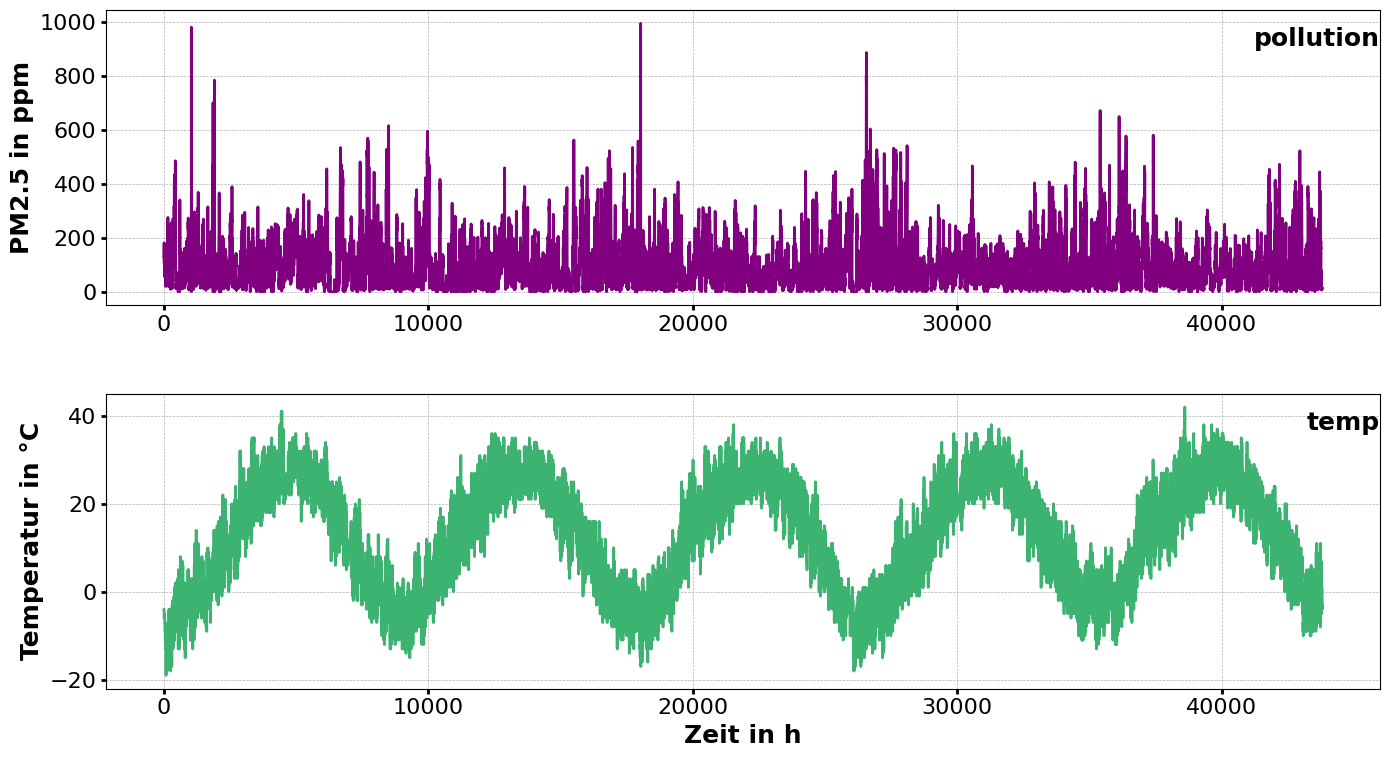
\includegraphics[width=0.8\textwidth]{Datenkorrelation_1.png}
  \caption{Datenkorrelation zwischen der Luftverschmutzung und Temperatur}
  \label{fig:fig1}
\end{figure}

Bei genauerer Betrachtung ist zu erkennen, dass sich die gewünschte Zielmetrik Luftverschmutzung antikorelliert verhält zur Temperatur. 
Zusätzlich ist bei Werten wie der Temperatur, Regen oder Windgeschwindigkeit eine Abhängigkeit zu Jahreszeiten erkennbar und somit existieren periodische Zyklen.

Generell werden alle \textbf{Features} mit Außnahme des Datums als Input benutzt. Dieses wird gelöscht und stattdessen eine Indexierung von 0 bis 43.800 Stunden verwendet, da dies die weitere Verarbeitung 
vereinfacht und zusätzlich Modellstabilität, sowie Skalierbarkeit positiv beeinflusst. 
Im nächsten Schritt steht die \textbf{Datenaufbereitung} im Fokus.
Zu Beginn ist eine Umwandlung der aktuellen Windrichtungen (NE, SE, NW, cv) in numerische Werte nötig, um sie für das LSTM nutzbar zu machen, wobei "cv" eine calm variable für Wind aus mehreren Richtungen darstellt.
Somit sind die neuen label encoded Werte wiefolgt: ['1', '2', '3', '4']. 
Danach wird eine Datentyp Standardisierung vorgenommen, die den Datentyp ``float32'' für alle Spalten festlegt. 
Somit wird sichergestellt, das alle Daten im gleichen Format vorliegen, was für viele Machine-Learning-Algorithmen wichtig ist.
Zusätzlich wird ein MinMaxScaler angewendet, der die Daten in einen Bereich von [0 , 1] skaliert und so für numerische Stabilität, sowie eine Vermeidung von Dominanz großer Werte sorgt. 
Im nächsten Schritt muss der Datensatz noch auf das bevorstehende LSTM Modell vorbereitet werden. 
Dabei wird der Datensatz als überwachtes Lernproblem formuliert und die Eingabevariablen werden normalisiert. 
Die dazugehörige Funktion zur Transformation und Normalisierung der Daten ist übernommen aus einem Machine-Learning Mastery Blog.\footcite[vgl.][1]{brownleeMultivariateTimeSeries2017}
Der Output enthält zusätzliche Spalten, die um eine Position verschoben sind, sodass mit den aktuellen Eingabespalten der jeweils nächste Wert vorhergesagt werden kann.
Eine Visualisierung der Transformation kann aus folgender Tab.\ref{tab:supervised_learning} entnommen werden.
\begin{table}[H]
  \centering
  \begin{tabular}{|c|c|}
  \hline
  \textbf{var1(t-1)} & \textbf{var1(t)} \\ \hline
  \rowcolor{cyan} 0.129779 & \cellcolor{yellow} 0.148893 \\ \hline
  \rowcolor{yellow} 0.148893 & \cellcolor{orange} 0.159960 \\ \hline
  \rowcolor{orange} 0.159960 & \cellcolor{green} 0.182093 \\ \hline
  \rowcolor{green} 0.182093 & \cellcolor{red} 0.138833 \\ \hline
  \rowcolor{red} 0.138833 & \cellcolor{pink} 0.109658 \\ \hline
  \end{tabular}
  \caption{Verschobene Werte für ein Supervised Learning Problem}
  \label{tab:supervised_learning}
\end{table}

Generell ist zu erkennen, dass alle Werte skaliert, normiert und nun auch als überwachtes Lernproblem dargestellt sind. 
Wie farbig zu erkennen ist, ist der aktuelle Wert der Luftverschmutzung var1(t-1) und der zu vorhersagende Wert var1(t) um eins versetzt und gewährleistet so eine Vorhersarge der Verschmutzung mit zeitlich vorangegangenen Daten.
Der letzte Schritt der Datenaufbereitung beinhaltet die Aufteilung der Daten in Trainingsdaten und Evaluationsdaten. 
Die Aufteilung ist klassisch durch 80\% Trainings- und 20\% Evaluationsdaten gekennzeichnet, wobei dies den oben genannten vier Jahren für Training und einem Jahr Evaluation entspricht.
Nachfolgend werden beide Teildatensätze nochmals in Eingabedaten, die alle Merkmale außer dem vorherzusagenden "Luftverschmutzung",
enthalten (train\_X, test\_X), und die vorherzusagenden Labels (train\_Y, test\_Y) unterteilt. 
Schlussendlich muss das Format der Daten noch in einem 3D-Array umgewandelt werden, da dies von einem LSTM benötigt wird.
Der 3D-Array sieht dabei wie folgt aus: Anzahl der Datenpunkte, Anzahl der Zeitschritte, Anzahl der Merkmale.


\section{Neuronales Netz}
\subsection{Zielmetrik}
Für das Training des Modells wird die Zielmetrik der mittleren quaratischen Abweichung benutzt.
Diese ist der Standard für Regressionsaufgaben, wie die Vorhersage der Luftverschmutzung. 
Der Mean Squared Error (MSE) wird durch die folgende Formel definiert:
\begin{equation}
MSE = \frac{1}{n} \sum_{i=1}^{n} (y_i - \hat{y}_i)^2,
\end{equation}
wobei \( y_i \) die tatsächlichen Werte und \( \hat{y}_i \) die vorhergesagten Werte sind. MSE eignet sich gut für Regressionsaufgaben, da sie große Fehler stärker gewichtet und somit das Modell dazu zwingt, größere Abweichungen zu minimieren, was zu präziseren Vorhersagen führt.\footcite[vgl.][672]{LinearRegressionVs}
Zusätzlich werden zwei weitere Metriken erhoben: Mean Absolute Error (MAE) und Root Mean Squared Error(RMSE), jedoch werden diese nicht als loss zum Training benutzt. 
Dennoch ermöglichen Sie ein besseres Verständnis über die Performance des Modells während und nach dem Training. 
Der MAE gibt hierbei die durchschnittliche Abweichung der absoluten Differenzen zwischen vorhergesagten und tatsächlichen Werten an.
Dies erlaubt Einblick in die durchschnittliche Größe der Fehler ohne zu stark auf Ausreißer zu reagieren und ermöglicht zudem ein einfacheres Verständnis,
da die Abweichung in derselben Einheit wie die Daten angegeben ist.
Der RMSE ist die Quadratwurzel des MSE und erfüllt den gleichen Zweck, jedoch steht er dadurch in der selben Einheit wie die Daten und ist somit leichter interpretierbar. 
Dennoch reagiert der RMSE stark auf größere Fehler, wie der eigentliche MSE.
Nutzen mehrerer Metriken ermöglicht zudem ein besseres Verständnis der Performance beim Hyperparametertuning. 
\subsection{Aufbau des Modells}
Das Benutzte neuronale Netzwerk ist ein sequentielles Modell zur Vorhersage von Luftverschmutzung bestehend aus insgesamt \textbf{fünf Schichten} und insgesamt 288,129 Parametern. 
Die Struktur ist inspiriert aus folgenden Papers, jedoch abgewandelt uns für diesen Datensatz und Aufgabenstellung angepasst\footnote{vgl.\cite{tanRegressionAnalysisPrediction2021}, p. 2-4; vgl.\cite{LinearRegressionVs}, p. 673}:

1. \textbf{LSTM-Schicht}: Diese Long Short Term Memory (LSTM) Schicht enthält 256 Neuronen und ist in der Lage, langfristige Abhängigkeiten in zeitlich geordneten Daten zu lernen. 
Die LSTM-Schicht verarbeitet die Eingabezeitreihen und extrahiert relevante Merkmale, die für die Vorhersage wichtig sind.

2. \textbf{Dense-Schicht}: Diese Schicht besteht aus 64 Neuronen und transformiert die von der LSTM-Schicht extrahierten Merkmale.
Sie ermöglicht es dem Modell, komplexe nichtlineare Beziehungen zu lernen.

3. \textbf{Dropout-Schicht}: Mit einer Rate von 0,25 wird ein zufälliger Prozentsatz der Neuronen während des Trainings deaktiviert.
Dies hilft, Overfitting zu vermeiden und die Generalisierungsfähigkeit des Modells zu verbessern.

4. \textbf{Batch-Normalisierungs-Schicht}: Diese Schicht normalisiert die Ausgaben der vorhergehenden Schicht. Sie beschleunigt das Training und verbessert die Stabilität des Modells,
indem sie die Verteilungen der Inputs zu den nachfolgenden Schichten konsistent hält.

5. \textbf{Finale Dense-Schicht}: Die letzte Schicht besteht aus einem einzelnen Neuron, das den vorhergesagten Wert der Luftverschmutzung ausgibt.
Diese Schicht aggregiert die verarbeiteten Informationen und liefert die endgültige Vorhersage.

Des Weiteren wird der \textbf{Adam-Optimizer} verwendet, um das Modell zu trainieren. Er kombiniert die Vorteile von AdaGrad und RMSProp, was zu einer schnellen und effizienten Konvergenz führt und somit die Optimierung des Modells verbessert.
Die \textbf{Loss-Funktion} des Modells, während dem Training, ist der Mean Squared Error (MSE), der große Fehler stärker gewichtet und somit die Vorhersagegenauigkeit verbessert.
Das Modell verwendet den  mit einer Lernrate von 0.001.

\subsection{Hyperparameter}
Durch die einzelnen Schichten gibt es etliche Hyperparameter, die getuned werden können, um die Genauigkeit des Modells zu erhöhen. 
Die Hyperparameter sind: 
\begin{table}[H]
  \centering
  \begin{tabular}{| m{5.5cm} | m{5.5cm} |}

  \hline
  \textbf{Hyperparameter} & \textbf{Benutzte Standardwerte} \\ \hline
  lstm\_units & 256 \\ \hline
  dense\_units\_1 & 64 \\ \hline
  dense\_units\_2 & 1 \\ \hline
  dropout\_rate & 0.25 \\ \hline
  learning\_rate & 0.001 \\ \hline

  epochs & 50 \\ \hline
  batch\_size & 128 \\ \hline
  activation\_function (Dense-Schichten) & Linear \\ \hline
  optimizer & Adam \\ \hline
  \end{tabular}
  \caption{Hyperparameter und deren Standardwerte}
  \label{tab:hyperparameters}
  \end{table}

\section{Evaluation des Trainings und Hyperparametertuning}
Generell wird für die Durchführung des Trainings Keras, als High-Level-API und Teil von Tensorflow zur Erstellung und Training von Deep-Learning-Modellen benutzt.
Das Ergebnis des nicht Hyperparameter optimierten Modells ist in folgender Abb.\ref{fig:ergebnis_vor} dargestellt:
\begin{figure}[H]
  \centering
  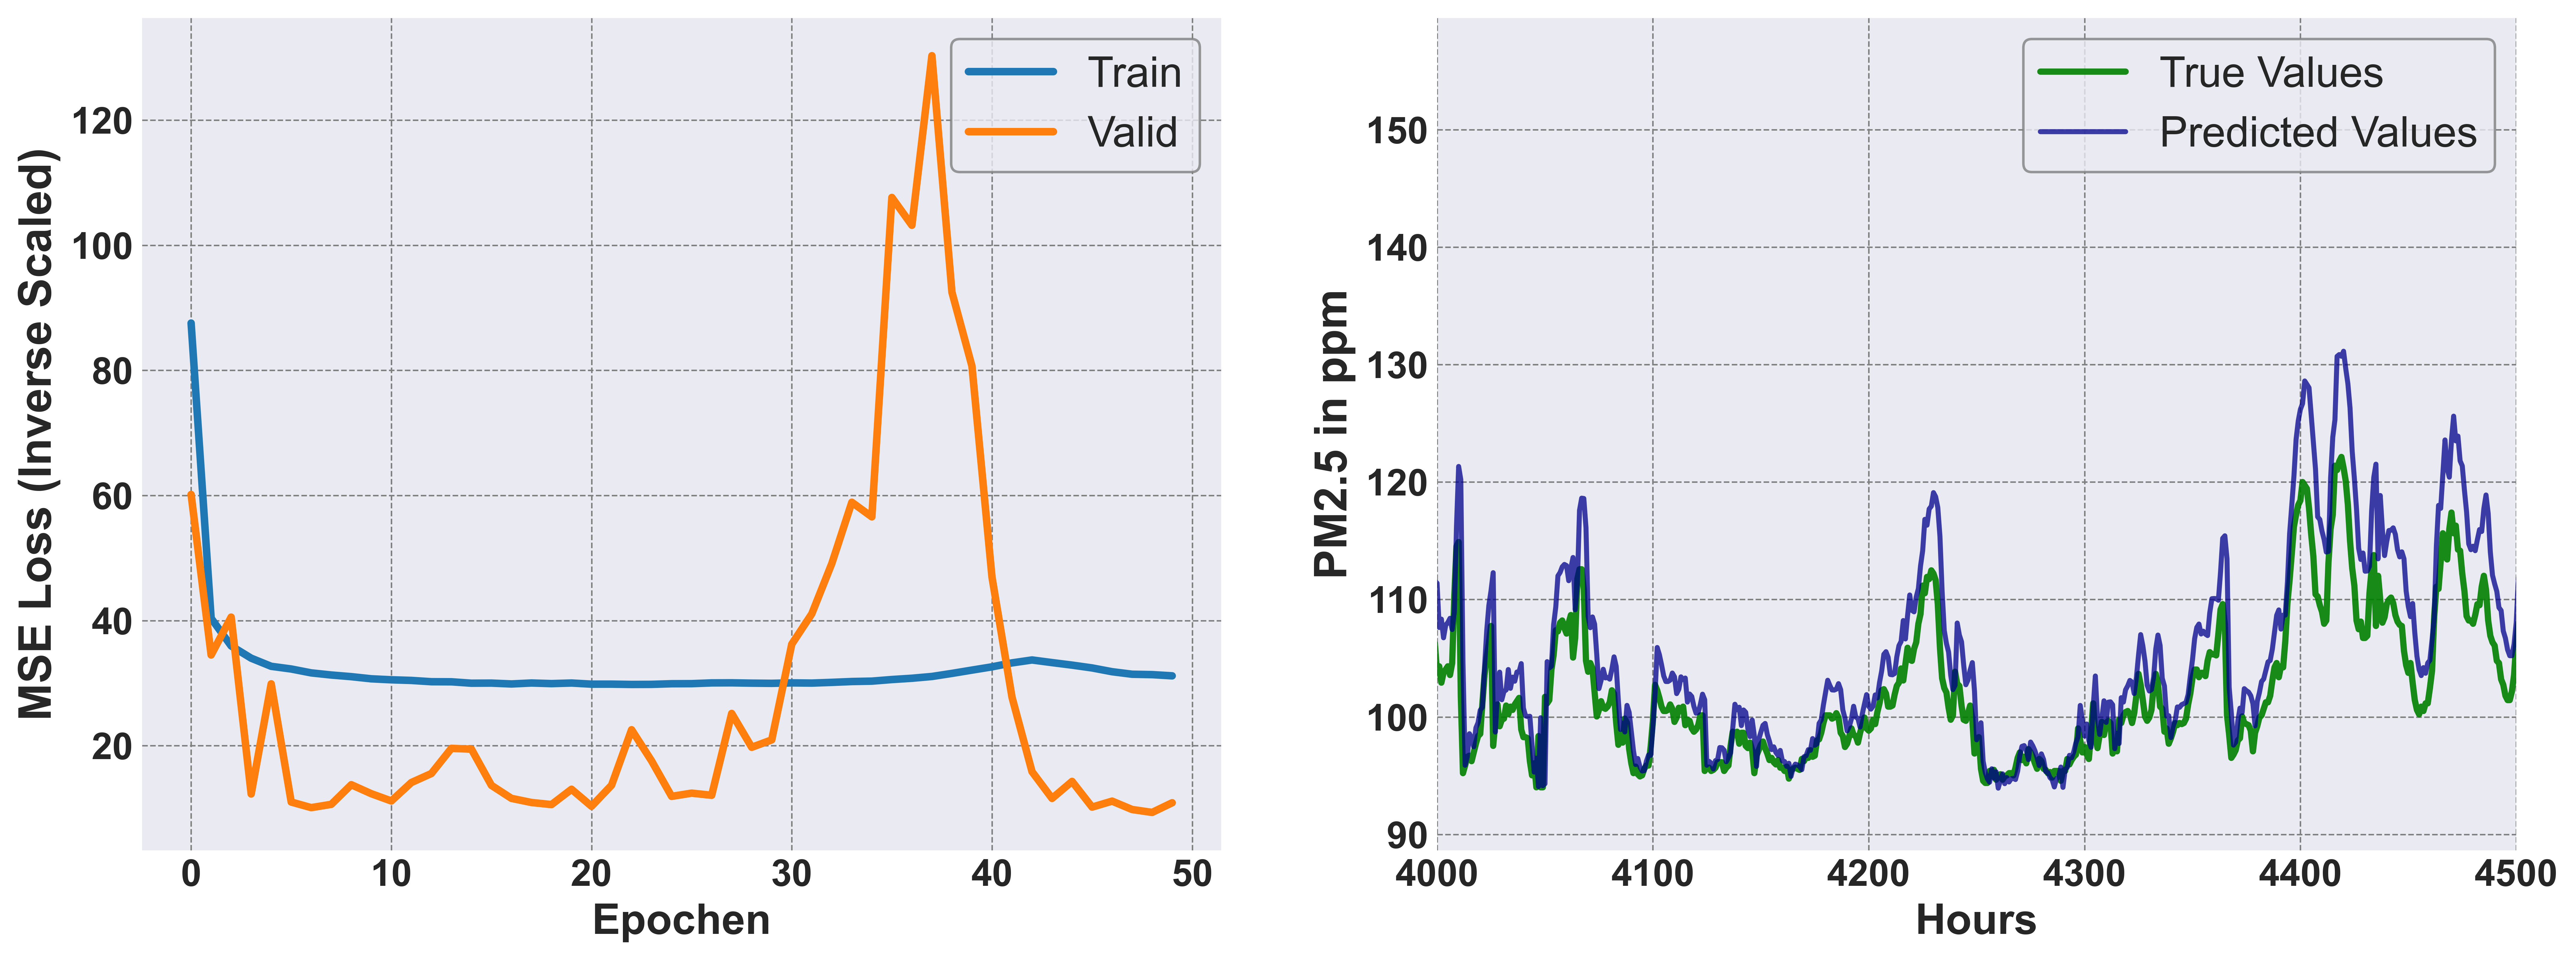
\includegraphics[width=1\textwidth]{output.png}
  \caption{Initialergebnisse}
  \label{fig:ergebnis_vor}
\end{figure}
In der linken Abb. ist zu erkennen, dass das Standardmodell nach 50 Trainingsepochen einen trainings-loss von 31.1 bezogen auf den MSE und sogar einen evaluation-loss von 10.8 erreicht, welche auf gute Performance deuten.
Hierbei ist zu erwähnen, dass der MSE Loss invertiert auf die Originalskala ist um eine korrekte und verständliche Interpretation zu ermöglichen. 
Des Weiteren sind ein paar Ausreißer in höheren Epochen des Trainings zu erkennen, welche sich jedoch gegen Ende des Trainings vaporisieren und nicht genauer untersucht werden.
Der Rechte plot veranschaulicht die vorhergesagten Werte im Vergleich zu den korrekten Luftverschmutzungswerten.
Hierfür wurde zudem der RMSE berechnet, indem die Differenzen zwischen den tatsächlichen Werten \(y_{\text{test\_true},i}\) und den vorhergesagten Werten \(\hat{y}_{\text{testPredict2},i}\) quadriert, gemittelt und dann die Quadratwurzel genommen wird.
Die Berechnung erfolgt somit nach folgender Formel:
\begin{equation}
RMSE = \sqrt{\frac{1}{n} \sum_{i=1}^{n} (y_{\text{test\_true},i} - \hat{y}_{\text{testPredict2},i})^2},
\end{equation}
mit dem Ergebnis von 3.29, was bedeutet, dass Vorhersagen hauptsächlich im Bereich von +-3.29ppm um die realen Werte schwanken. 

Im nächsten Schritt findet ein Hyperparametertuning mit dem ML Lifecycle Mgt Tool "MLFLow" statt.
Da es etliche, Hyperparameter gibt und der Zeitaufwand zu enorm ist, alle Hyperparameter zu betrachten, wird sich auf die Batch Size konzentriert.
Diese gibt an, wie viele Trainingsbeispiele in einem einzelnen Vorwärts-/Rückwärtsdurchlauf verarbeitet werden. 
Speziell wird die Batch Size zu Beginn auf 2 gesetzt und anschließend verdoppelt, bis eine Batch Size von 256 erreicht wird. 
Der Hintergrund hierbei ist, dass ein Vielfaches von 2 oftmals recheneffizieter ist und mehr Hardwarekompatibilität bietet.
Als Ausnahme sind drei Zwischenschritte bei 100, 150 und 200 eingefügt, um zu große Abstände der Batch Sizes vorzubeugen. 
MLFlow benötigt hierbei einen Experimentnamen, unter dem die Runs gespeichert werden, und zudem die zu speichernden Parameter, wie etwa der MSE Loss oder RMSE und natürlich die einzelnen Hyperparameter. 
Ebenfalls muss hier darauf geachtet werden, dass die Evaluationsmetrik auf die Originalskala inversiert werden kann, um Vergleichbarkeit und Interpretierbarkeit zu schaffen.
Das Ergebnis des Hyperparametertunings ist in folgender Abb.\ref{fig:ergebnis_nach} ersichtlich:
\begin{figure}[H]
  \centering
  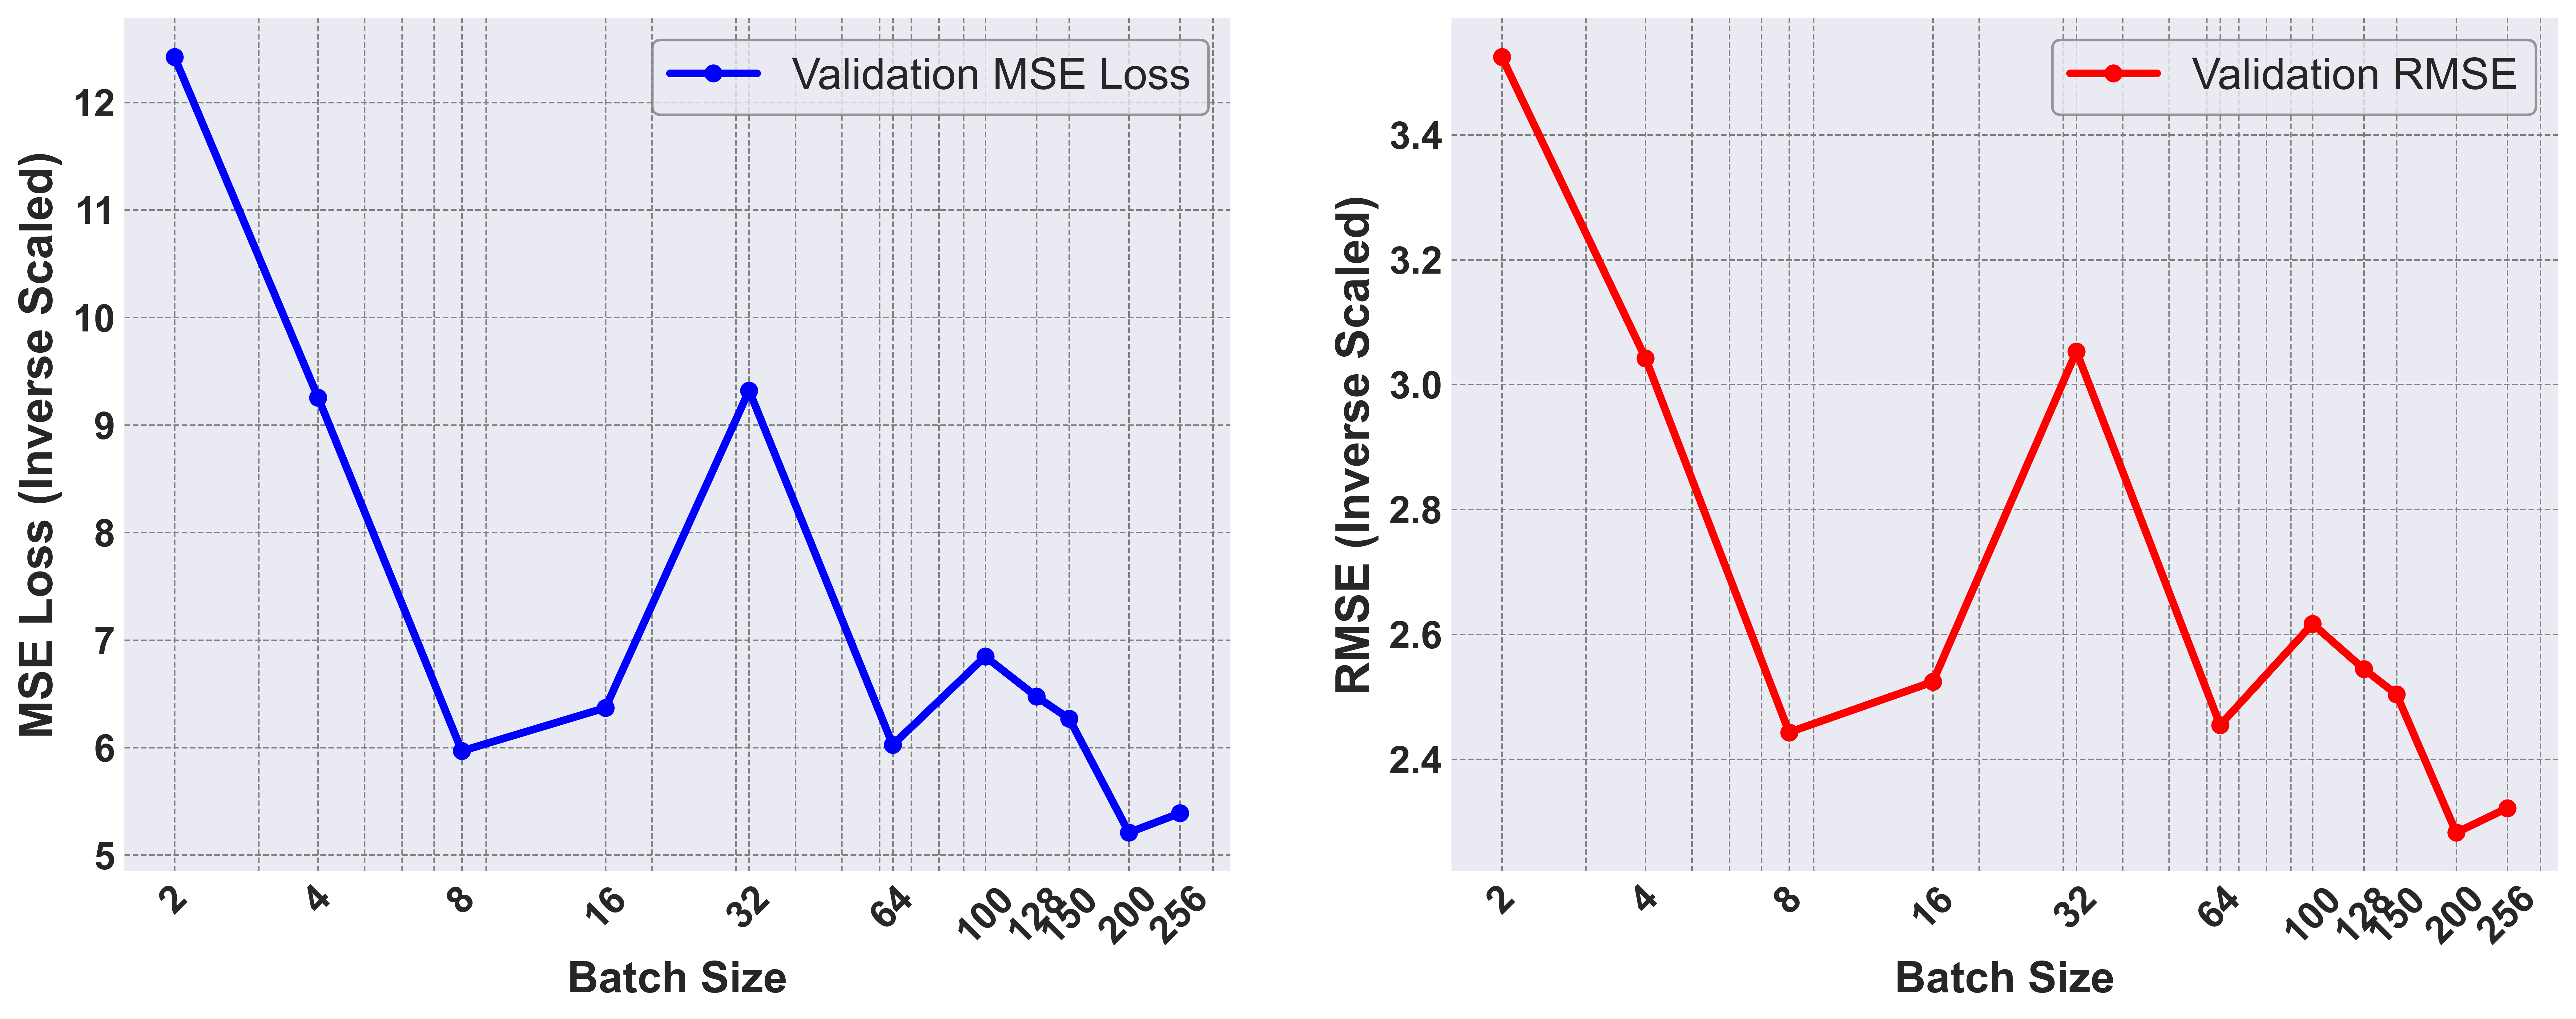
\includegraphics[width=0.95\textwidth]{Ergebnisse NACH Hyperparametertuning.png}
  \caption{Hyperparametertuning der Batch Size}
  \label{fig:ergebnis_nach}
\end{figure}
Aufgeführt in blau ist der MSE Loss und in rot der besser interpretierbare RMSE. 
Es ist zu erkennen, dass das Modell mit höheren Batch-Sizes, speziell einer Batch-Size von 200, seine Genauigkeit von den ursprünglichen +-3.29 (RMSE) 
auf +-2.28 (RMSE) senken kann, was einer Verbesserung von 31\% entspricht.
Diese Verbesserung durch die Verwendung größerer Batch-Sizes ist darauf zurückzuführen, dass mehr Daten aus der Vergangenheit genutzt werden, wodurch die Luftverschmutzung am Folgetag genauer vorhergesagt werden kann.

\section{Fazit}

Die Studie zeigt, dass ein LSTM-Modell effektiv zur Vorhersage der Luftverschmutzung genutzt werden kann.
Durch die Aufbereitung und Skalierung der Daten, sowie der Anwendung von Feature Engineering, konnte ein robustes Modell entwickelt werden.
Die Hyperparameteroptimierung, speziell der Batch Size, führte zudem zu einer signifikanten Steigerung der Vorhersagegenauigkeit, wobei der RMSE von ursprünglich +-3.29 ppm auf +-2.28 ppm gesenkt wurde.
Dies entspricht einer Genauigkeitsverbesserung von 31\%.
Zusammenfassend stellt das Modell eine wertvolle Ressource zur Unterstützung politischer Entscheidungsträger und Umweltbehörden dar, um die Planung von Maßnahmen zur Luftqualitätskontrolle zu verbessern.


%Bibliography
\printbibliography

% \bibliographystyle{unsrt}  
% \bibliography{Machine_Learning_Project}  


\end{document}